\section{Auswertung}
\subsection{Wheatstonesche Messbrücke}
Der erste Bestandteil des Versuchs bestand darin mit Hilfe der Wheatstoneschen Brückenschaltung die Werte von zwei verschiedenen Widerständen zu bestimmen.
Die zu bestimmenden Bauteile sind die Widerstände $R_\text{13}$ und $R_\text{14}$.
Die gemessenen Werte für $R_2$, $R_3$ und $R_4$ sind in der folgenden Tabelle dargestellt.

\begin{table}[h!]
    \begin{center}
      \caption{Messung der Widerstände.}
      \label{tab:Tabelle 1}
      \begin{tabular}{c|c|c} 
        \multicolumn{3}{c}{R Wert 13} \\
        \textbf{$R_2 / \Omega$ } & \textbf{$R_3 / \Omega$} & \textbf{$R_4 / \Omega$}\\
        \hline
        332 & 485 & 515\\
        664 & 318 & 682\\
        1000 & 235 & 765\\
        \multicolumn{3}{c}{R Wert 14} \\
        \hline
        332 & 728 & 272\\
        664 & 571 & 429\\
        1000 & 468 & 532\\
      \end{tabular}
    \end{center}
\end{table}

$R_2$ hat dabei einen relativen Fehler von $\pm 0.2 \%$, während der Quotient
\begin{equation*}
    \frac{R_\text{3}}{R_\text{4}}
\end{equation*}
des Potentiometers einen relativen Fehler von $\pm 0.5 \%$ hat.
Es ergibt sich mit der Gausschen Fehlerfortpflanzung allgemein folgender Fehler.
\begin{equation}
    \Delta f = \sqrt{\sum \limits_{i=1}^{N} \left (\frac{\partial f}{\partial x_i} \cdot \Delta x_i \right)^2}
\end{equation}
Mit den gemessenen Werten und nach (5) lässt sich jeweils ein Wert für $R_x$ bestimmen, woraus sich dann der Mittelwert wie folgt berechnen lässt.
\begin{equation}
    \overline{x} = \frac{1}{N} \sum_{i=1}^N x_i
\end{equation}
Bei der Berechnung des Mittelwerts ergibt sich allerdings ein Fehler, der über die Varianz $V$ bestimmt werden kann.
Aus der Varianz lässt sich der Fehler des Mittelwerts bestimmen, wenn man die Standardabweichung als
\begin{equation*}
    \sigma = \sqrt{V}
\end{equation*}
definiert.
Also ergibt sich für den Fehler des Mittelwerts
\begin{equation}
    \Delta \overline{x} = \frac{\sigma}{\sqrt{N(N-1)}} = \sqrt{\frac{\sum \limits_{i=1}^N (x_i-\overline{x})^2}{N(N-1)}}
\end{equation}
Nach (15), (16), (17) und folgender Gausschen Fehlerfortpflanzung lassen sich nun die Werte für $R_\text{13}$, $R_\text{14}$ und deren Fehler bestimmen.
\begin{equation}
    \Delta R_x = \sqrt{\left (\frac{\partial R_x}{\partial R_2}\cdot \Delta R_2 \right )^2 + \left (\frac{\partial R_x}{\partial \left (\frac{R_3}{R_4}\right )} \cdot \left (\Delta \frac{R_3}{R_4}\right )\right )^2}
\end{equation}
Für die Werte $R_\text{13}$ und $R_\text{14}$ ergeben sich
\begin{equation}
    \overline{R_\text{13}} = \SI{309,819 \pm 0,963}{\Omega}\notag
\end{equation} 
\begin{equation}
    \overline{R_\text{14}} = \SI{884,024 \pm 2,749}{\Omega}\notag
\end{equation}
Zusätzlich kommt noch der Fehler des Mittelwertes hinzu.
Hierbei beträgt \\
\begin{equation*}
    \Delta \overline{R_\text{13}} = \SI{0,963}{\Omega}
\end{equation*}
und
\begin{equation*}
    \Delta \overline{R_\text{14}} = \SI{1,483}{\Omega}
\end{equation*}.

\subsection{Kapazitätsmessbrücke}
Die Kapazitätsmessbrücke ermöglicht es, Verlustwiderstände und Kapazitäten von Kondensatoren zu bestimmen.
Zunächst werden Kapazitäten unter der Annahme berechnet, dass der gesuchte Kondensator $C_x$ und der Messkondensator $C_2$ als ideal angenommen werden.
Die folgende Tabelle zeigt die Messwerte auf.

\begin{table}[h!]
    \begin{center}
      \caption{Messung der Kapazitäten.}
      \label{tab:Tabelle 2}
      \begin{tabular}{c|c|c} 
        \multicolumn{3}{c}{C Wert 3} \\
        \textbf{$C_2 / nF$ } & \textbf{$R_3 / \Omega$} & \textbf{$R_4 / \Omega$}\\
        \hline
        399 & 485 & 515\\
        450 & 513 & 487\\
        750 & 636 & 364\\
        \multicolumn{3}{c}{C Wert 14} \\
        \textbf{$C_2 / nF$ } & \textbf{$R_3 / \Omega$} & \textbf{$R_4 / \Omega$}\\
        \hline
        399 & 203 & 797\\
        450 & 222 & 778\\
        750 & 323 & 677\\
      \end{tabular}
    \end{center}
\end{table}
Nach (6) aus der Theorie lassen sich die Kapazitäten der als ideal angenommenen Kondensatoren bestimmen.
Außerdem wird der Mittelwert aus den jeweils drei berechneten Werten nach (16) und dem entsprechenden Fehler des Mittelwertes aus (17) gebildet.
Hinzu kommt der Fehler der Bauteile, der durch die Gaussche Fehlerfortpflanzung bestimmt wird.
\begin{equation}
    \Delta C_x = \sqrt{\left (\frac{\partial C_x}{\partial C_2}\cdot \Delta C_2 \right )^2 + \left (\frac{\partial C_x}{\partial \left (\frac{R_3}{R_4}\right )} \cdot \left (\Delta \frac{R_3}{R_4}\right )\right )^2}
\end{equation}
Hierbei bleibt der Fehler des Potentiometers gleich und die des Kondensators liegt bei $\pm 0.2 \%$.
Damit ergeben sich folgende Mittelwerte für die Kapazität.
\begin{equation}
    \overline{C_\text{3}} = \SI{426,706 \pm 1,327}{nF} \notag 
\end{equation}
\begin{equation}
    \overline{C_\text{14}} = \SI{1571,842 \pm 4,887}{nF} \notag 
\end{equation}

Hinzufügend wird noch der Fehler des Mittelwerts bestimmt
Hierbei beträgt \\
\begin{equation*}
    \Delta \overline{C_\text{3}} = \SI{0.938}{nF}
\end{equation*}
und
\begin{equation*}
    \Delta \overline{C_\text{14}} = \SI{1,752}{nF}
\end{equation*}.\\
Zusätzlich wird noch ein realer Kondensator betrachtet, der eine Kapazität und einen Verlustwiderstand enthält.
In der folgenden Tabelle sind die gemessenen Werte abgebildet.
\begin{table}[h!]
    \begin{center}
      \caption{Messung des RC-Bauteils(8).}
      \label{tab:Tabelle 3}
      \begin{tabular}{c|c|c|c} 
        \multicolumn{3}{c}{C Wert 3} \\
        \textbf{$C_2 / nF$ } & \textbf{$R_2 / \Omega$} & \textbf{$R_3 / \Omega$} & \textbf{$R_4 / \Omega$}\\
        \hline
        399 & 426 & 573 & 427\\
        450 & 378 & 601 & 399\\
        750 & 229 & 714 & 286\\
      \end{tabular}
    \end{center}
\end{table}

Nach (6) und (7) aus der Theorie und der Gausschen Fehlerfortpflanzung (18) und (19) lassen sich die jeweiligen Werte für das Bauteil berechnen.
Der Mittelwert wird mit (16) gebildet und es ergeben sich folgende Werte
\begin{equation}
    \overline{R_\text{8}} = \SI{570,909 \pm 1,775}{\Omega} \notag
\end{equation}
\begin{equation}
    \overline{C_\text{8}} = \SI{298,836 \pm 0,929}{nF} \notag
\end{equation}
Durch (17) lassen sich die Fehler der Mittelwerte auf
\begin{equation*}
    \Delta \overline{R_\text{8}} = \SI{0,445}{\Omega}
\end{equation*}
und
\begin{equation*}
    \Delta \overline{C_\text{8}} = \SI{0.515}{nF}
\end{equation*} bestimmen.

\subsection{Induktivitätsmessbrücke}
Hier wird die Induktivität und der Verlustwiderstand einer Spule bestimmt.
Der Fehler des Potentiometers bleibt erneut gleich und der relative Fehler der anderen Bauteile beträgt $\pm 0.2 \%$.
Durch (8) und (15) folgt
\begin{equation}
    \Delta L_x = \sqrt{\left (\frac{\partial L_x}{\partial L_2}\cdot \Delta L_2 \right )^2 + \left (\frac{\partial L_x}{\partial \left (\frac{R_3}{R_4}\right )} \cdot \left (\Delta \frac{R_3}{R_4}\right )\right )^2}
\end{equation}
Zusätzlich wird die Fehlerfortpflanzung (18) des Widerstands verwendet.
Es ergeben sich folgende Werte für den Verlustwiderstand und die Induktivität der Spule.
\begin{equation}
    R_\text{19} = \SI{105,149 \pm 0,566}{\Omega} \notag
\end{equation}
\begin{equation}
    L_\text{19} = \SI{26,753 \pm 0,144}{mH} \notag
\end{equation}

\subsection{Maxwell-Brücke}
Die relativen Fehler der Bauteile werden von der Induktivitätsbrücke übernommen.
Des Weiteren wird die Gaussche Fehlerfortpflanzung (18) für den Widerstand übernommen.
Anders als bei der Induktivität, dort ergibt sich nach (10) und (15) folgende Fehlerfortpflanzung.
\begin{equation}
    \Delta L_x = \sqrt{\left (\frac{\partial L_x}{\partial R_2}\cdot \Delta R_2 \right )^2 + \left (\frac{\partial L_x}{\partial R_3} \cdot \Delta R_3\right )^2 + \left (\frac{\partial L_x}{\partial C_4} \cdot \Delta C_4\right )^2 }
\end{equation}
Der Widerstand und die Induktivität werden mit (10) und (11) auf folgende Werte bestimmt.
\begin{equation}
    R_\text{19} = \SI{114,331 \pm 4,856}{\Omega} \notag
\end{equation}
\begin{equation}
    L_\text{19} = \SI{27,553 \pm 0,831}{mH} \notag
\end{equation}

\subsection{Wien-Robinson-Filter}
Im Folgenden wird die Frequenzabhängigkeit des Schwingkreises bestimmt.
Hierbei ist 
\begin{equation*}
    R' = \SI{332}{\Omega}
\end{equation*},
\begin{equation*}
    R = \SI{1000}{\Omega}
\end{equation*} und 
\begin{equation*}
    C = \SI{993}{nF}
\end{equation*}.

\subsubsection{Sperrfrequenz}
Zunächst wird die Frequenz des Sinusgenerators, bei der die Brückenspannung $U_\text{Br}$ verschwindet, theoretisch mit (12) berechnet.
Dabei ist
\begin{equation*}
    \omega_0 = \frac{1}{RC}
\end{equation*}.
Es ergibt sich also für die Sperrfrequenz des Schwingkreises
\begin{equation}
    \nu_0 = \frac{\omega_0}{2\pi} = \frac{1}{2\pi RC}
\end{equation}
Die Sperrfrequenz beträgt somit
\begin{equation*}
    \nu_0 = \SI{160,277}{Hz}
\end{equation*}.
Im Folgenden sind die Werte aus Tabelle 4 und die theoretische Kurve, die mit (13) und
\begin{equation*}
    \Omega = \frac{\nu}{\nu_0}
\end{equation*} berechnet wurde, aufgetragen.
Dabei ist $\Omega$ gegen den natürichen Logarithmus des Quotienten $\frac{U_\text{Br}}{U_S}$ aufgetragen.
Es fällt auf, dass die Kurven sehr gut übereinstimmen.
Die experimentelle Sperrfrequenz lässt sich somit auf folgenden Wert bestimmen.
\begin{equation}
    \nu_0 = \SI{157,523 \pm 1,246}{Hz} \notag
\end{equation}

\begin{table}[h!]
    \begin{center}
      \caption{Frequenzabhängigkeit.}
      \label{tab:Tabelle 4}
      \begin{tabular}{c|c|c} 
        \textbf{$\nu / Hz$ } & \textbf{$U_\text{Br} / mV$} & \textbf{$U_\text{S} / V$}\\
        \hline
        80 & 1090 & 7,10\\
        90 & 1050 & 7,10\\
        100 & 709 & 7,10\\
        110 & 531 & 7,10\\
        120 & 405 & 7,10\\
        130 & 260 & 7,10\\
        140 & 145 & 7,10\\
        150 & 36 & 7,10\\
        160 & 39 & 7,00\\
        170 & 139 & 7,00\\
        180 & 217 & 7,00\\
        190 & 306 & 7,00\\
        200 & 375 & 7,00\\
        210 & 459 & 7,00\\
        220 & 511 & 6,95\\
        230 & 582 & 6,95\\
        240 & 630 & 6,95\\
        250 & 700 & 6,95\\
        260 & 752 & 6,95\\
        270 & 809 & 6,95\\
      \end{tabular}
    \end{center}
\end{table}

\begin{figure}[H]
  \centering
  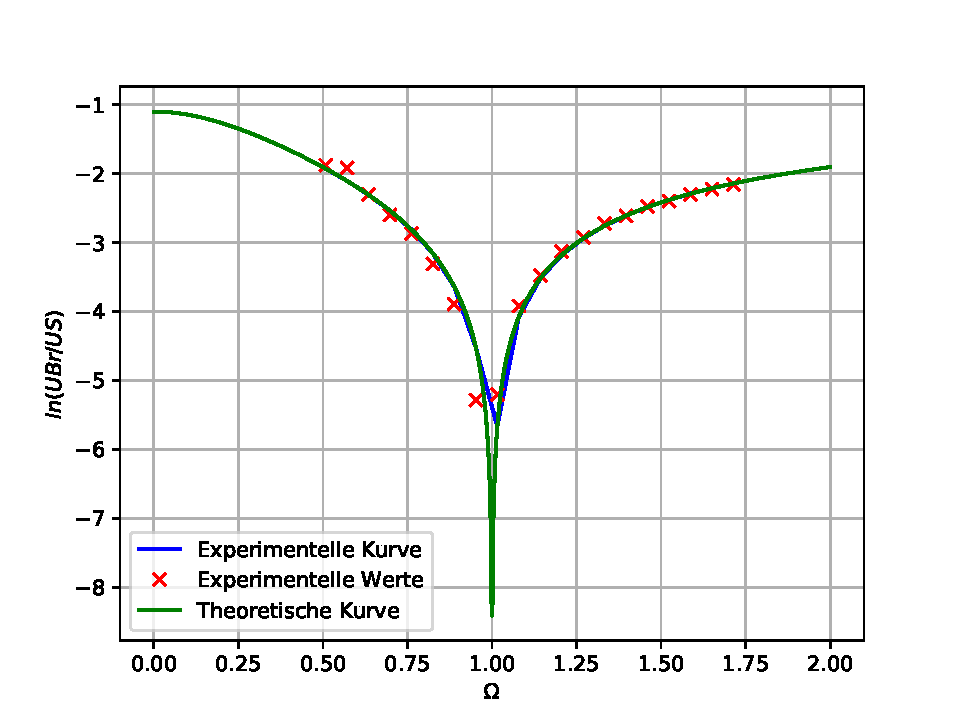
\includegraphics[height=10cm]{Auswertung/Frequenz_neu.pdf}
  \caption{Frequenzbhängigkeit.}
  \label{fig:Frequenz}
\end{figure}

\subsubsection{Klirrfaktor}
Der Klirrfaktor lässt sich aus den ungewollten Oberwellen des Sinusgenerators bestimmen und allgemein wie folgt berechnen.
\begin{equation}
    k = \frac{\sqrt{U_2^2 + U_3^2 + ...}}{U_1}
\end{equation}
Es wird genähert, dass die Summe der Oberwellen aus (23) nur aus der zweiten Oberwelle besteht.
Für die zweite Oberwelle ergibt sich außerdem folgende Formel
\begin{equation}
    U_2 = \frac{U_\text{Br}}{f(2)}
\end{equation}

Hierbei wird (13) als Funktion f bezeichnet und
\begin{equation*}
    \Omega = 2
\end{equation*} gesetzt.
Es ergibt sich
\begin{equation}
	f(2) = \sqrt{\frac{1}{9}\frac{(2^2 - 1)^2}{(1-2^2)^2 + 9 \cdot 2^2}} = \frac{\sqrt{5}}{15} \notag
\end{equation}
Damit lässt sich $U_2$ aus der Brückenspannung $U_\text{Br}$ bei der Sperrfrequenz bestimmen.
$U_1$ beschreibt in (23) die Spannung des Sinusgenerators $U_\text{S,min}$ bei der Sperrfrequenz $\nu_0$, die durch die Oberwellen entsteht.
Eingesetzt ergibt sich für den Klirrfaktor Folgendes.

\begin{equation}
    k = \frac{U_2}{U_1} = \frac{U_\text{Br}}{f(2) \cdot U_\text{S,min}} = \frac{15}{\sqrt{5}} \cdot \frac{U_\text{Br}}{U_\text{S,min}} \notag
\end{equation}

Der Klirrfaktor des verwendeten Sinusgenerators liegt bei $3,45\%$.
